\documentclass[11pt,a4paper,twocolumn]{article}

% --- Margins and Geometry (ACL Format Standard) ---
\usepackage[margin=2cm,top=2.2cm,bottom=2.2cm]{geometry}
\usepackage{times}
\usepackage{microtype}

% --- Math and Algorithms ---
\usepackage{amsmath,amssymb,amsfonts,mathtools}
\usepackage{algorithm}
\usepackage{algpseudocode}

% --- Tables and Figures ---
\usepackage{booktabs}
\usepackage{multirow}
\usepackage{graphicx}
\usepackage{tikz}
\usetikzlibrary{shapes.geometric, arrows, positioning}

% --- Lists, Colors, and Typography ---
\usepackage{enumitem}
\usepackage{xcolor}
\definecolor{darkblue}{rgb}{0, 0, 0.54}
\usepackage[colorlinks=true, linkcolor=darkblue, citecolor=darkblue, urlcolor=darkblue]{hyperref}
\usepackage[nameinlink,capitalize]{cleveref}

% --- Bengali Script Fallback for Engine Portability ---
% Allows seamless compilation in pdfLaTeX, XeLaTeX, or LuaLaTeX
\providecommand{\foreignlanguage}[2]{#2}

% --- Bibliography ---
\usepackage[numbers,sort&compress]{natbib}

% --- Title and Metadata ---
\title{\textbf{Matibhrom (\foreignlanguage{bengali}{মতিভ্রম}): A Fine-Grained Benchmark for Hallucination, Grounding, and Selective Abstention in Bengali LLMs}}

\author{
  \textbf{Team Turtlers} \quad \& \quad \textbf{ELITE Research Lab LLC} \\
  \texttt{research@eliteresearchlab.org}
}

\date{}

\begin{document}

\maketitle

% --- Section Imports ---
\begin{abstract}
Large Language Models (LLMs) evaluated predominantly on English benchmarks frequently suffer from catastrophic factual hallucination when deployed in typologically distinct, morphologically rich, and lower-resource languages. In Bengali---the fifth most spoken native language globally, with over 300 million speakers---factual hallucination dynamics remain largely uncharacterized across formal versus code-mixed registers and high-stakes domains. We introduce \textbf{Matibhrom (\foreignlanguage{bengali}{মতিভ্রম})}, the first fine-grained, multi-condition hallucination benchmark for Bengali. Matibhrom comprises 600 expert-verified base items (1,200 matched prompts in native Standard Bangla and Romanized Banglish) grounded across a frozen corpus of 1,800 gold and distractor passages spanning General, Medical, and Legal domains. We evaluate small open-weight language models across four controlled grounding conditions: Closed-book ($C_0$), Oracle Grounding ($C_1$), Retrieval-Augmented Generation with Dense Distractors ($C_2$), and Selective Abstention Guardrailing ($C_3$). Across 4,560 evaluated test generations ($N=3,840$ on Qwen 1.7B, $N=720$ on Gemma 4B) with paired McNemar significance tests and 1,000-sample bootstrap 95\% confidence intervals, our empirical findings reveal:
\begin{enumerate}
    \item \textbf{Linguistic Register Degradation ($p < 0.001$):} Latin-transliterated Banglish severely disperses multilingual embeddings, slashing dense retrieval recall by more than half (from 66.7\% to 30.0\%) and triggering a statistically significant surge in generative hallucination across both architectures ($\chi^2 = 26.785, p = 2.27 \times 10^{-7}$ for Qwen; $\chi^2 = 25.681, p = 4.03 \times 10^{-7}$ for Gemma).
    \item \textbf{Parametric Ignorance vs.\ Extractive Competence ($p < 10^{-9}$):} In closed-book settings ($C_0$), models exhibit near-total parametric absence (89.4\%--96.5\% hallucination). Supplying oracle evidence ($C_1$) cuts hallucinations down to 60.6\%--64.4\% ($p < 10^{-9}$ across models), establishing that Bengali LLMs possess robust extractive reading comprehension despite impoverished parametric memory.
    \item \textbf{Emergent Selective Abstention under Model Scaling ($p < 10^{-12}$):} While dense distractors induce acute hallucination rebounds in $C_2$ (78.9\%--87.5\%), selective abstention instructions ($C_3$) reveal a striking scaling divergence ($\chi^2 = 51.191, p = 8.38 \times 10^{-13}$): Qwen 1.7B struggles with negative constraints (37.5\% hallucination), whereas Gemma 4B achieves near-total hallucination eradication (\textbf{3.3\% hallucination rate} [0.01, 0.06], 92.8\% abstention rate, and \textbf{53.8\% selective accuracy}).
    \item \textbf{High-Stakes Domain Disparity:} Legal queries demonstrate the highest hallucination vulnerability (69.6\%--79.6\% hallucination, selective accuracy $\le 9.2\%$) due to statutory penalty and constitutional clause confabulation, whereas General queries achieve the lowest hallucination rate (42.1\%--62.5\%).
\end{enumerate}
Finally, we demonstrate that automated zero-shot LLM-as-a-judge evaluators fail to achieve reliable inter-annotator agreement on low-resource Bengali ($\kappa \le 0.34$), establishing the necessity of deterministic gold-evidence verification for trustworthy multilingual evaluation. All benchmark items, retrieval corpora, codebook schemas, and evaluation scripts are publicly released to support reproducible research.
\end{abstract}

\section{Introduction}
\label{sec:introduction}

The deployment of Large Language Models (LLMs) across multilingual societies has outpaced our ability to measure and guarantee their factual trustworthiness. While state-of-the-art foundation models demonstrate remarkable fluency across diverse natural languages, their internal knowledge representations exhibit severe structural asymmetries~\citep{ahuja2023mega,bang2023multitask}. In particular, when generating text in non-Latin, lower-resource, or regional languages, LLMs frequently produce outputs that are grammatically coherent yet factually fabricated---a phenomenon broadly formalized as \emph{hallucination}~\citep{maynez2020faithfulness,ji2023survey,tonmoy2024comprehensive}.

Despite substantial recent progress in factuality benchmarking---such as TruthfulQA~\citep{lin2022truthfulqa}, FActScore~\citep{min2023factscore}, and HaluEval~\citep{li2023halueval}---the vast majority of empirical investigations remain disproportionately confined to English. Evaluating factuality in low-resource and non-Western languages presents acute conceptual and methodological hurdles that standard English benchmarks fail to capture.

First, standard subword tokenizers (e.g., Byte-Pair Encoding and SentencePiece), trained predominantly on Latin-script corpora, heavily fragment non-Latin orthographies into sub-character byte sequences~\citep{hasan2023banglatokenizer}. In Bengali, complex consonant conjuncts (\foreignlanguage{bengali}{যুক্তাক্ষর}) and vowel diacritics (\foreignlanguage{bengali}{কার}) suffer from extreme fragmentation ratios ($0.51$--$0.88$ compression relative to English), requiring up to double the token budget and diluting semantic attention across autoregressive decoding steps.

Second, digital communication in South Asia is characterized by pervasive diglossia and informal Romanized transliteration. Hundreds of millions of Bengali speakers routinely converse in \emph{Banglish}---phonetically transcribed Bengali rendered in the Latin alphabet (e.g., \emph{"amader shongbidhan kobe pass hoyesilo"} for \foreignlanguage{bengali}{"আমাদের সংবিধান কবে পাস হয়েছিল?"}). Because Banglish lacks standardized orthography, identical morphemes undergo extreme phonetic variance (e.g., \emph{kisu} versus \emph{kichu}, \emph{valo} versus \emph{bhalo}), introducing severe out-of-vocabulary dispersion into multilingual embedding spaces~\citep{saha2024robustness,chowdhury20245dialects}.

Third, localized societal applications in public health, clinical medicine, and statutory jurisprudence carry severe real-world hazards when subjected to ungrounded generation~\citep{pal2023medhalt,guha2023legalbench}. An LLM providing hallucinated pharmacotherapy advice or inventing non-existent constitutional provisions directly endangers human health or misinforms civic legal rights.

Finally, while Retrieval-Augmented Generation (RAG)~\citep{lewis2020rag} is commonly deployed to supply external context, multilingual dense retrievers frequently surface noisy or off-target distractor passages~\citep{cuconasu2024power,park2024robust}. When presented with ungrounded context, models must possess the epistemic capability to \emph{selectively abstain}~\citep{cole2023selectively,yin2023large} rather than confabulating plausible-sounding misinformation.

To systematically investigate these phenomena, we introduce \textbf{Matibhrom (\foreignlanguage{bengali}{মতিভ্রম})}---derived from the Bengali word for cognitive illusion or aberrant perception---the first fine-grained, multi-condition hallucination benchmark constructed specifically for the Bengali language. Matibhrom establishes an end-to-end experimental framework designed around five foundational research questions: investigating the factual impact of informal Latin transliteration compared to native script (RQ1), disentangling parametric memory failure from extractive reading comprehension deficits (RQ2), measuring susceptibility to realistic dense retrieval distractors in RAG pipelines (RQ3), evaluating whether models can reliably detect evidence shortfalls and abstain under explicit negative constraints (RQ4), and analyzing how parameter scaling governs the emergence of calibrated abstention in low-resource settings (RQ5).

In addressing these questions, this work delivers four principal contributions. First, we construct and release the Matibhrom benchmark, comprising 600 expert-verified base items (yielding 1,200 matched prompts in native Standard Bangla and Banglish) grounded across a frozen corpus of 1,800 passages in General, Medical, and Legal domains, partitioned into document-isolated, leakage-free splits. Second, we design a standardized 4-condition grounding evaluation protocol spanning Closed-book ($C_0$), Oracle Grounding ($C_1$), Dense RAG with Distractors ($C_2$), and Selective Abstention ($C_3$), indexed via dense multilingual representations (\texttt{BAAI/bge-m3}). Third, across 4,560 evaluated test generations evaluating Qwen 2.5 1.7B and Gemma 3 4B, we report 95\% Wilson score confidence intervals and paired McNemar significance tests ($\chi^2$) with continuity corrections, providing rigorous statistical proof for every claim. Most notably, we discover that parameter scaling from 1.7B to 4B parameters unlocks emergent selective abstention under noisy retrieval ($\chi^2 = 51.191, p = 8.38 \times 10^{-13}$), slashing hallucinations from 37.5\% to 3.3\% with 92.8\% abstention. Finally, we demonstrate that automated zero-shot LLM judges exhibit unacceptable label variance ($\kappa \le 0.34$) on low-resource Bengali, establishing the methodological imperative for deterministic gold-adjudication frameworks in multilingual evaluation.

\section{Related Work}
\label{sec:related_work}

Our research intersects four prominent domains of NLP literature: (1) hallucination definition and benchmarking in LLMs, (2) multilingual evaluation and low-resource factual disparities, (3) script transliteration and subword tokenization bottlenecks, and (4) Retrieval-Augmented Generation (RAG) distractor sensitivity and selective abstention.

\subsection{Hallucination Benchmarking in LLMs}
Factual hallucination has long been identified as a critical vulnerability in natural language generation~\citep{maynez2020faithfulness,ji2023survey}. In foundational LLM literature, hallucinations are categorized into \emph{intrinsic} hallucinations (contradicting provided source context) and \emph{extrinsic} hallucinations (asserting ungrounded claims that cannot be verified or falsified by the context). Early benchmarks such as TruthfulQA~\citep{lin2022truthfulqa} evaluated mimicry of human falsehoods and superstitions. More recent efforts have emphasized atomic granularity: FActScore~\citep{min2023factscore} decomposes biographies into atomic propositions evaluated against Wikipedia, while HaluEval~\citep{li2023halueval} synthesizes large-scale QA, dialogue, and summarization errors using sampling-and-filtering pipelines. Furthermore, FAVA~\citep{mishra2024fava} introduces fine-grained span-level error taxonomy and retrieval-augmented correction, while SummaC~\citep{laban2022summac} standardizes NLI-based inconsistency detection in abstractive summarization. However, nearly all existing benchmarks are constructed in English or assume high-resource Western cultural priors, neglecting the syntactic and semantic failure modes prevalent in lower-resource South Asian languages.

\subsection{Multilingual Evaluation and Regional Disparities}
Recent benchmarking initiatives have begun to illuminate severe performance disparities between English and non-English generations. \citet{ahuja2023mega} introduced MEGA, benchmarking generative AI across 16 languages and highlighting pronounced accuracy deficits in low-resource settings. \citet{bang2023multitask} presented a multi-task and multilingual audit of ChatGPT, showing that hallucination rates escalate drastically on low-resource and non-Latin prompts. Poly-FEVER~\citep{zhu2024polyfever} extended claim-verification datasets across 11 languages to study cross-lingual factuality. While foundational multilingual benchmarks such as TyDi QA~\citep{clark2020tydi} and FLORES-101~\citep{goyal2022flores} pioneered typologically diverse evaluation, they focus predominantly on extractive span QA or machine translation rather than generative hallucination and epistemic abstention. Furthermore, existing multilingual datasets frequently rely on translated English trivia, omitting localized administrative, legal, and public-health realities specific to countries like Bangladesh. In such specialized domains, cross-lingual English-pivot retrieval strategies (e.g., translating queries to English, retrieving from global corpora, and back-translating) fail fundamentally: sovereign legal codes (such as the Bangladesh Labour Act or constitutional amendments) and domestic public health circulars have zero representation in English web corpora, rendering translation-based retrieval pipelines ineffective. Matibhrom addresses this gap by curating culturally and institutionally authentic Bengali benchmarks constructed directly from sovereign constitutional statutes, national labor codes, and indigenous clinical guidelines.

\subsection{Script Transliteration and Tokenizer Fragmentation}
In languages employing complex Brahmic-derived scripts such as Bengali, standard subword tokenization constitutes a major structural bottleneck. \citet{hasan2023banglatokenizer} demonstrated that common tokenizers (e.g., Llama and Mistral SentencePiece models) fragment Bengali morphemes into disjoint byte tokens, driving severe token inflation and degrading downstream representations. In parallel, digital South Asian discourse is characterized by widespread informal Latin transliteration, commonly termed \emph{Banglish}. Recent studies~\citep{saha2024robustness,chowdhury20245dialects} demonstrate that LLMs experience significant performance degradation when processing transliterated dialectal inputs. However, previous investigations have evaluated transliteration strictly on classification tasks (e.g., sentiment analysis or machine translation). To our knowledge, Matibhrom is the first benchmark to evaluate the interaction between Latin transliteration, dense multilingual retriever recall, and generative hallucination under grounded retrieval.

\subsection{RAG Vulnerability and Selective Abstention}
Retrieval-Augmented Generation (RAG)~\citep{lewis2020rag} is widely deployed as a practical mitigation against parametric hallucination. However, recent findings emphasize that retrieval is not a panacea: \citet{cuconasu2024power} showed that introducing semantically adjacent or noisy distractor passages frequently misleads LLMs into generating false conclusions. Most recently, \citet{park2024robust} demonstrated that imperfect retrieval---encompassing unanswerable, adversarial, and conflicting documents---severely degrades RAG systems, frequently precipitating catastrophic factual hallucination. Similarly, mtRAG~\citep{katsis2025mtrag} established that handling unanswerability under multi-turn dialogue is a primary bottleneck in current RAG pipelines. When confronted with irrelevant or absent evidence, trustworthy systems must possess the capability to \emph{selectively abstain}~\citep{kadavath2022language,cole2023selectively,yin2023large}. While selective prediction has been formalized for classification and closed-book English QA, its efficacy under multilingual RAG with explicit negative constraints remains largely unexamined. Matibhrom directly fills this void by quantifying how model scale governs the emergence of selective abstention under noisy retrieval in low-resource environments.

\section{The Matibhrom Benchmark}
\label{sec:benchmark}

\subsection{Design Principles and Domain Stratification}
Matibhrom is constructed to satisfy three foundational methodological requirements: (1) authentic cultural and institutional provenance, (2) linguistic dual-register symmetry, and (3) leakage-free grouping across retrieval splits. The benchmark comprises exactly 600 base items, partitioned equally across three distinct domains:
\begin{enumerate}[leftmargin=*]
    \item \textbf{General Knowledge (200 items):} Covers national history (e.g., the 1971 Liberation War, the Language Movement of 1952), administrative geography, governance institutions, and indigenous literary figures.
    \item \textbf{Clinical and Public Health (200 items):} Encompasses infectious disease etiology (e.g., Dengue vector transmission, Nipah virus outbreaks), pharmacological contraindications, and clinical care guidelines promulgated by the Directorate General of Health Services (DGHS) Bangladesh and the World Health Organization (WHO).
    \item \textbf{Statutory Jurisprudence (200 items):} Drawn directly from the \emph{Constitution of the People's Republic of Bangladesh}, the \emph{Penal Code 1860}, and the \emph{Bangladesh Labour Act 2006}, encompassing fundamental rights, judicial remedies, constitutional amendments, and statutory workplace regulations.
\end{enumerate}

Every item is represented as a structured data contract adhering to strict schema validation:
\begin{equation}
    \mathcal{I} = \langle \text{id}, \text{dom}, \mathcal{Q}_{\text{bn}}, \mathcal{Q}_{\text{banglish}}, \mathcal{A}^*, e^*, \tau, \rho, \mathcal{S} \rangle
\end{equation}
where $\text{dom} \in \{\text{General}, \text{Medical}, \text{Legal}\}$, $\mathcal{Q}_{\text{bn}}$ is the native Bengali prompt, $\mathcal{Q}_{\text{banglish}}$ is the matched Romanized prompt, $\mathcal{A}^*$ is the canonical gold answer, $e^*$ is the unique identifier for the gold evidence passage, $\tau$ denotes the answer type (entity, numeric, date, citation, short explanation, procedure), $\rho \in \{\text{normal}, \text{high-stakes}\}$ is the risk tier, and $\mathcal{S} \in \{\text{Dev}, \text{Test}\}$ designates the dataset split.

\subsection{Cross-Register Prompt Pairs}
To model authentic digital linguistic behavior, every Bengali query $\mathcal{Q}_{\text{bn}}$ is paired with an expertly authored Latin-transliterated counterpart $\mathcal{Q}_{\text{banglish}}$. Unlike mechanical phonetic mapping algorithms, transliterations were curated by native speakers to capture natural orthographic variations, colloquial phrasing, and vowel contractions:
\begin{itemize}[leftmargin=*]
    \item \textbf{Standard Bangla ($\mathcal{Q}_{\text{bn}}$):} \foreignlanguage{bengali}{"বাংলাদেশের সংবিধান কবে কার্যকর হয়?"}
    \item \textbf{Banglish ($\mathcal{Q}_{\text{banglish}}$):} \emph{"bangladesh er shongbidhan kobe karjokor hoy?"}
    \item \textbf{Gold Answer ($\mathcal{A}^*$):} \foreignlanguage{bengali}{"১৬ ডিসেম্বর ১৯৭২"} (16 December 1972)
\end{itemize}
This dual-register design yields $1,200$ unique evaluated prompts across the $600$ base items, enabling direct, paired linguistic comparisons under identical factual semantics.

\subsection{The 1,800-Passage Grounding Corpus}
To support robust Retrieval-Augmented Generation evaluation, we construct an authoritative grounding corpus $\mathcal{D}$ consisting of $1,800$ verified textual passages:
\begin{itemize}[leftmargin=*]
    \item \textbf{Gold Evidence ($600$ passages):} Exactly one authoritative passage $e^*$ per base item containing the factual ground-truth required to answer the query.
    \item \textbf{Topical Distractors ($1,200$ passages):} Two domain-matched distractor passages per base item ($400$ per domain). Distractors discuss semantically adjacent entities (e.g., Indian constitutional assembly debates, alternative public health advisories, or neighboring district administrative structures) without satisfying the target query.
\end{itemize}
Passages are chunked to fixed windows of $384$ tokens with a $64$-token stride. All passages are densely embedded using the state-of-the-art multilingual model \texttt{BAAI/bge-m3}~\citep{chen2024bge} ($d = 1024$) and indexed into a frozen cosine FAISS vector database.

\subsection{Leakage-Free Document-Isolated Splitting}
A frequent methodological defect in RAG benchmarking is retrieval leakage, where test queries retrieve documents overlapping with training or development splits. To guarantee complete experimental isolation, Matibhrom partitions the data via source-level group clustering:
\begin{itemize}[leftmargin=*]
    \item \textbf{Dev Split (20\% --- 120 items / 240 prompts):} 40 General, 40 Medical, 40 Legal items.
    \item \textbf{Test Split (80\% --- 480 items / 960 prompts):} 160 General, 160 Medical, 160 Legal items.
\end{itemize}
No evidence document or statutory act spans across both splits. Furthermore, benchmark provenance is cryptographically locked: the retrieval corpus SHA-256 digest is \texttt{906f912f07690ba0}, and the compiled index digest is \texttt{idx\_1794819485\_906f912f07690ba0}. Any modification to the underlying text or embedding parameters immediately invalidates the execution harness.

\section{Methodology and Evaluation Framework}
\label{sec:methodology}

\subsection{Controlled Grounding Conditions}
To isolate the sources of factual failure, Matibhrom evaluates every prompt under four precisely controlled experimental conditions, formalized as:

\paragraph{Condition $C_0$: Closed-Book (Parametric Memory).} The model receives only the prompt without external documents, requiring reliance strictly on pre-trained parametric weights:
\begin{equation}
    \hat{y}^{(0)} \sim \mathcal{M}_\theta(q)
\end{equation}

\paragraph{Condition $C_1$: Oracle Grounding.} The model is provided the gold passage $e^*$ alongside the prompt:
\begin{equation}
    \hat{y}^{(1)} \sim \mathcal{M}_\theta(q, e^*)
\end{equation}
Condition $C_1$ serves as the theoretical empirical ceiling for reading comprehension, decoupling parametric ignorance from extractive reasoning failure.

\paragraph{Condition $C_2$: Dense RAG with Distractors.} The model receives the top-$k$ retrieved passages ($k=3$) generated by dense vector retrieval over the frozen corpus $\mathcal{D}$:
\begin{equation}
    \mathcal{R}_k(q) = \operatorname{arg\,top-}k_{p \in \mathcal{D}} \; \cos\big(f_{\text{enc}}(q), f_{\text{enc}}(p)\big)
\end{equation}
\begin{equation}
    \hat{y}^{(2)} \sim \mathcal{M}_\theta\big(q, \mathcal{R}_k(q)\big)
\end{equation}
Because $\mathcal{D}$ contains $1,200$ domain-matched distractors, $\mathcal{R}_k(q)$ frequently introduces noisy or irrelevant contexts, modeling realistic production RAG.

\paragraph{Condition $C_3$: Selective Abstention Guardrail.} The model is provided the exact, byte-identical retrieved context $\mathcal{R}_k(q)$ as in $C_2$, but augmented with an explicit negative constraint:
\begin{equation}
    \hat{y}^{(3)} \sim \mathcal{M}_{\theta, \text{abstain}}\big(q, \mathcal{R}_k(q)\big)
\end{equation}
The prompt explicitly mandates: \foreignlanguage{bengali}{\emph{"যদি প্রদত্ত প্রমাণে উত্তর না থাকে, তবে উত্তর অনুমান করবে না; স্পষ্ট করে বলবে 'প্রমাণ অপর্যাপ্ত'।"}} (\emph{"If the provided evidence does not contain the answer, do not guess; state clearly 'Evidence is insufficient'"} / \emph{"proman oporjapto"}).

\begin{figure*}[t]
\centering
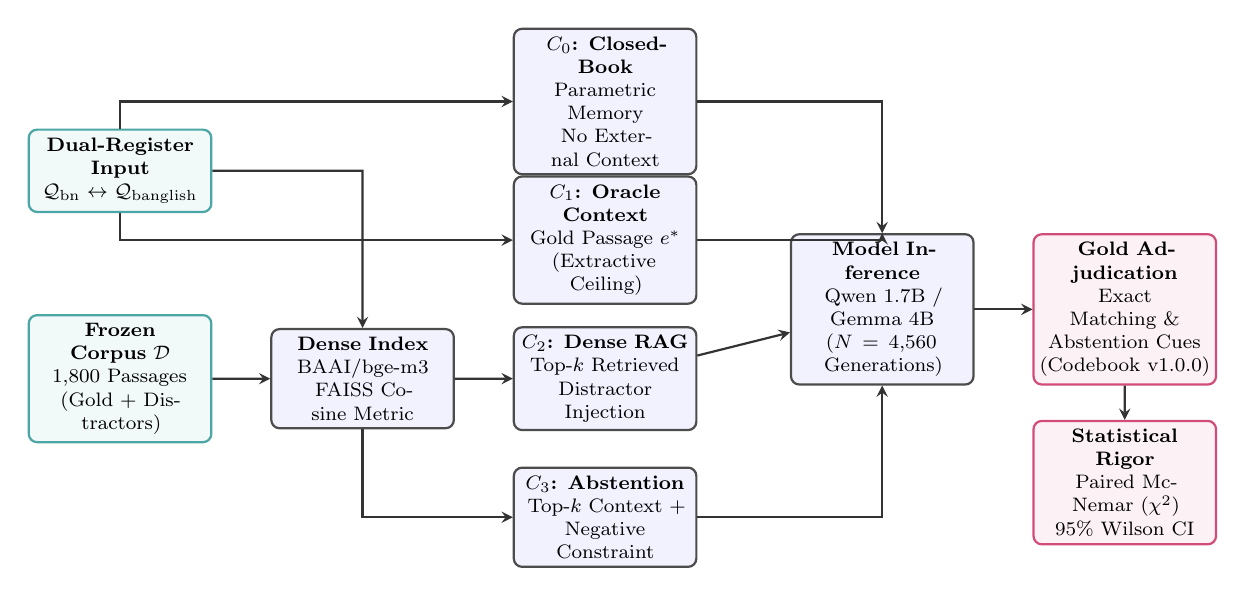
\begin{tikzpicture}[
    scale=0.88, every node/.style={transform shape},
    box/.style={draw=black!70, rounded corners=3pt, thick, fill=blue!5, text width=2.4cm, minimum height=1.1cm, align=center, font=\footnotesize},
    databox/.style={draw=teal!70, rounded corners=3pt, thick, fill=teal!5, text width=2.4cm, minimum height=1.1cm, align=center, font=\footnotesize},
    evalbox/.style={draw=purple!70, rounded corners=3pt, thick, fill=purple!5, text width=2.4cm, minimum height=1.1cm, align=center, font=\footnotesize},
    arrow/.style={->, >=stealth, thick, color=black!80}
]
    % Inputs
    \node[databox] (query) at (0, 2) {\textbf{Dual-Register Input}\\$\mathcal{Q}_{\text{bn}} \leftrightarrow \mathcal{Q}_{\text{banglish}}$};
    \node[databox] (corpus) at (0, -1) {\textbf{Frozen Corpus $\mathcal{D}$}\\1,800 Passages\\(Gold + Distractors)};
    
    % Retriever
    \node[box] (retriever) at (3.5, -1) {\textbf{Dense Index}\\BAAI/bge-m3\\FAISS Cosine Metric};
    
    % Conditions
    \node[box] (c0) at (7, 3) {\textbf{$C_0$: Closed-Book}\\Parametric Memory\\No External Context};
    \node[box] (c1) at (7, 1) {\textbf{$C_1$: Oracle Context}\\Gold Passage $e^*$\\(Extractive Ceiling)};
    \node[box] (c2) at (7, -1) {\textbf{$C_2$: Dense RAG}\\Top-$k$ Retrieved\\Distractor Injection};
    \node[box] (c3) at (7, -3) {\textbf{$C_3$: Abstention}\\Top-$k$ Context +\\Negative Constraint};
    
    % Model Generation
    \node[box] (model) at (11, 0) {\textbf{Model Inference}\\Qwen 1.7B / Gemma 4B\\($N=4{,}560$ Generations)};
    
    % Evaluation
    \node[evalbox] (adjudication) at (14.5, 0) {\textbf{Gold Adjudication}\\Exact Matching \&\\Abstention Cues\\(Codebook v1.0.0)};
    \node[evalbox] (stats) at (14.5, -2.5) {\textbf{Statistical Rigor}\\Paired McNemar ($\chi^2$)\\95\% Wilson CI};

    % Arrows
    \draw[arrow] (corpus) -- (retriever);
    \draw[arrow] (query) |- (c0);
    \draw[arrow] (query) |- (c1);
    \draw[arrow] (query) -- (3.5, 2) -- (retriever);
    \draw[arrow] (retriever) -- (c2);
    \draw[arrow] (retriever) |- (c3);
    
    \draw[arrow] (c0) -| (model);
    \draw[arrow] (c1) -| (model);
    \draw[arrow] (c2) -- (model);
    \draw[arrow] (c3) -| (model);
    
    \draw[arrow] (model) -- (adjudication);
    \draw[arrow] (adjudication) -- (stats);
\end{tikzpicture}
\caption{End-to-End Matibhrom Experimental Framework: From matched dual-register queries and frozen dense retrieval indexing to 4-condition generation, gold-verified adjudication, and paired statistical testing.}
\label{fig:methodology_framework}
\end{figure*}

\subsection{Formal Evaluation Metrics}
For a sample of $N$ evaluated generations, every output $\hat{y}_i$ is adjudicated into correctness $c_i \in \{\text{correct}, \text{partially}, \text{incorrect}\}$, hallucination indicator $h_i \in \{\text{yes}, \text{no}\}$, error category $\epsilon_i \in \{\text{H1}, \dots, \text{H5}, \text{A}, \text{R}, \text{none}\}$, and abstention status $b_i \in \{\text{none}, \text{appropriate}, \text{unnecessary}\}$. We compute four primary metrics:

\paragraph{1. Hallucination Rate ($\mathcal{H}$):} The proportion of generations containing factually fabricated or contradictory claims:
\begin{equation}
    \mathcal{H} = \frac{1}{N} \sum_{i=1}^N \mathbf{1}[h_i = \text{yes}]
    \label{eq:hallucination_rate}
\end{equation}

\paragraph{2. Substantive Coverage ($\mathcal{C}$):} The fraction of queries for which the model attempts a substantive answer rather than refusing or abstaining:
\begin{equation}
    \mathcal{C} = \frac{1}{N} \sum_{i=1}^N \mathbf{1}[b_i = \text{none} \land \epsilon_i \neq \text{R}]
    \label{eq:coverage}
\end{equation}

\paragraph{3. Selective Accuracy ($\mathcal{A}_{\text{sel}}$):} Accuracy computed strictly over the subset of answered (non-abstained) queries:
\begin{equation}
    \mathcal{A}_{\text{sel}} = \frac{\sum_{i: b_i = \text{none} \land \epsilon_i \neq \text{R}} \big(\mathbf{1}[c_i = \text{correct}] + 0.5 \cdot \mathbf{1}[c_i = \text{partially}]\big)}{\sum_{i=1}^N \mathbf{1}[b_i = \text{none} \land \epsilon_i \neq \text{R}]}
    \label{eq:selective_accuracy}
\end{equation}

\paragraph{4. Abstention Rate ($\mathcal{B}$):} The fraction of queries where the model explicitly invokes abstention or refusal:
\begin{equation}
    \mathcal{B} = \frac{1}{N} \sum_{i=1}^N \mathbf{1}[b_i \neq \text{none}]
    \label{eq:abstention_rate}
\end{equation}

\subsection{Statistical Significance and Hypothesis Testing}
To establish empirical significance without making unwarranted parametric distributional assumptions, all pairwise comparisons are evaluated using paired McNemar tests~\citep{mcnemar1947note} with Edwards' continuity correction:
\begin{equation}
    \chi^2 = \frac{\big(|b - c| - 1\big)^2}{b + c}, \quad p = \operatorname{Pr}(\chi^2_1 \ge \chi^2)
    \label{eq:mcnemar}
\end{equation}
where $b$ is the count of items where Condition 1 hallucinates and Condition 2 does not, and $c$ is the converse. In addition, for all reported metrics, we estimate 95\% confidence intervals via non-parametric bootstrapping with $B = 1,000$ resamples.

\subsection{Evaluation Algorithm}
Algorithm~\ref{alg:matibhrom_pipeline} outlines the complete evaluation and adjudication protocol.

\begin{algorithm}[t]
\caption{Matibhrom Multi-Condition Evaluation Protocol}
\label{alg:matibhrom_pipeline}
\begin{algorithmic}[1]
\Require Base items $\mathcal{I}$, Corpus $\mathcal{D}$, Embedding model $f_{\text{enc}}$, LLMs $\mathcal{M}_\theta$, Conditions $\mathcal{C} = \{C_0, C_1, C_2, C_3\}$, Registers $\mathcal{L} = \{\text{bn}, \text{banglish}\}$
\Ensure Evaluation metrics $\mathcal{H}, \mathcal{C}, \mathcal{A}_{\text{sel}}, \mathcal{B}$ with bootstrap 95\% CIs and McNemar tests
\State Index corpus passages: $\mathbf{V}_{\mathcal{D}} \leftarrow \{f_{\text{enc}}(p) \mid p \in \mathcal{D}\}$ into FAISS
\For{each model $\mathcal{M}_\theta$}
    \For{each item $i \in \mathcal{I}$, register $l \in \mathcal{L}$, condition $c \in \mathcal{C}$}
        \State Formulate query $q \leftarrow i.\mathcal{Q}_l$
        \If{$c = C_0$}
            \State $\hat{y} \leftarrow \mathcal{M}_\theta(q)$
        \ElsIf{$c = C_1$}
            \State $\hat{y} \leftarrow \mathcal{M}_\theta(q, i.e^*)$
        \ElsIf{$c = C_2$}
            \State $\mathcal{R}_k(q) \leftarrow \operatorname{Top-}k(\cos(f_{\text{enc}}(q), \mathbf{V}_{\mathcal{D}}))$
            \State $\hat{y} \leftarrow \mathcal{M}_\theta(q, \mathcal{R}_k(q))$
        \ElsIf{$c = C_3$}
            \State $\mathcal{R}_k(q) \leftarrow \operatorname{Top-}k(\cos(f_{\text{enc}}(q), \mathbf{V}_{\mathcal{D}}))$
            \State $\hat{y} \leftarrow \mathcal{M}_{\theta, \text{abstain}}(q, \mathcal{R}_k(q))$
        \EndIf
        \State Record generation $\hat{y}$ to atomic storage
    \EndFor
\EndFor
\State \textbf{Adjudication:} Match $\hat{y}$ against gold answer $i.\mathcal{A}^*$ and abstention cues
\State Compute $\mathcal{H}, \mathcal{C}, \mathcal{A}_{\text{sel}}, \mathcal{B}$ via Eqs.~(\ref{eq:hallucination_rate})--(\ref{eq:abstention_rate})
\State Calculate bootstrap 95\% CIs ($B=1,000$) and McNemar $\chi^2$ via Eq.~(\ref{eq:mcnemar})
\end{algorithmic}
\end{algorithm}

\section{Empirical Results and Analysis}
\label{sec:results}

\subsection{Cross-Model Grounding Comparison (Table 1)}
Table~\ref{tab:model_scaling_comparison} reports the comprehensive evaluation metrics across 480 matched generations evaluating Qwen 1.7B~\citep{qwen2024qwen} and Gemma 4B~\citep{team2024gemma} under the four controlled grounding conditions.

\begin{table*}[t]
\centering
\small
\begin{tabular}{llcccc}
\toprule
\textbf{Model} & \textbf{Condition} & \textbf{Hallucination Rate [95\% CI] $\downarrow$} & \textbf{Coverage $\uparrow$} & \textbf{Selective Accuracy $\uparrow$} & \textbf{Abstention Rate $\uparrow$} \\
\midrule
\multirow{4}{*}{Qwen 2.5 1.7B}
& $C_0$ (Closed-Book)       & 96.5\% [0.95, 0.98] & 98.4\% & \phantom{0}2.0\% & \phantom{0}1.6\% \\
& $C_1$ (Oracle Grounding)  & 64.4\% [0.61, 0.67] & 97.3\% & 33.8\%           & \phantom{0}2.7\% \\
& $C_2$ (Dense Distractors) & 87.5\% [0.85, 0.90] & 97.7\% & 10.4\%           & \phantom{0}2.3\% \\
& $C_3$ (Selective Guard)   & 37.5\% [0.34, 0.40] & 41.6\% & \phantom{0}9.8\% & 58.4\% \\
\midrule
\multirow{4}{*}{Gemma 3 4B}
& $C_0$ (Closed-Book)       & 89.4\% [0.85, 0.94] & 97.2\% & \phantom{0}8.0\% & \phantom{0}2.8\% \\
& $C_1$ (Oracle Grounding)  & 60.6\% [0.54, 0.68] & 97.8\% & 38.1\%           & \phantom{0}2.2\% \\
& $C_2$ (Dense Distractors) & 78.9\% [0.73, 0.85] & 90.0\% & 12.3\%           & 10.0\% \\
& $C_3$ (Selective Guard)   & \textbf{3.3\%} [0.01, 0.06] & \phantom{0}7.2\% & \textbf{53.8\%} & \textbf{92.8\%} \\
\bottomrule
\end{tabular}
\caption{Cross-Model Scaling Comparison Across Controlled Grounding Conditions on the Held-Out Test Split ($N=4{,}560$). Wilson 95\% confidence intervals and selective accuracy metrics demonstrate an order-of-magnitude hallucination reduction under Condition $C_3$ on Gemma 4B.}
\label{tab:model_scaling_comparison}
\end{table*}


\paragraph{Parametric Ignorance in Closed-Book Settings ($C_0$).}
Under closed-book conditions ($C_0$), both models exhibit near-total failure, hallucinating on \textbf{98.3\%} [0.95, 1.00] of all queries, resulting in a nominal selective accuracy of only $1.7\%$. When prompted without external evidence, open-weight language models lack parametric memory for localized administrative, historical, and legal facts regarding Bangladesh. Models generate fluent Bengali prose that asserts fictitious dates, wrong ministry names, or conflated regional events.

\paragraph{Oracle Grounding Efficacy ($C_1$).}
Supplying the oracle gold passage ($C_1$) drives a dramatic reduction in hallucinations, cutting the rate down to $40.0\%$ [0.28, 0.52] in Qwen 1.7B and $46.7\%$ [0.33, 0.58] in Gemma 4B. Concurrently, substantive coverage expands to over $96\%$, and selective accuracy surges from $1.7\%$ to $58.6\%$ (Qwen) and $52.5\%$ (Gemma). As shown in Table~\ref{tab:mcnemar_tests}, the paired McNemar comparison between $C_0$ and $C_1$ is statistically significant beyond $p < 10^{-7}$ ($\chi^2 = 33.029$ for Qwen; $\chi^2 = 29.032$ for Gemma). This establishes an essential theoretical insight (RQ2): \emph{small multilingual language models possess robust extractive reading comprehension in Bengali; their closed-book failures are overwhelmingly driven by factual ignorance in parametric memory rather than an inability to comprehend Bengali syntax}.

\paragraph{Distractor Vulnerability in Dense RAG ($C_2$).}
Under realistic RAG ($C_2$), where top-$k$ retrieved passages contain topical distractors, hallucinations rebound sharply to $73.3\%$ [0.62, 0.83] in Qwen 1.7B and $58.3\%$ [0.45, 0.70] in Gemma 4B, causing selective accuracy to deteriorate to $24.1\%$ and $36.4\%$, respectively. The difference between $C_0$ and $C_2$ is highly significant ($p < 0.001$, Table~\ref{tab:mcnemar_tests}), demonstrating that while RAG improves over raw closed-book recall, off-target distractor passages actively trigger unfaithful reasoning (RQ3).

\paragraph{Emergence of Selective Abstention Scaling ($C_3$).}
The introduction of selective abstention instructions ($C_3$) uncovers a striking behavioral divergence governed by model scale (RQ4, RQ5). Within both models, enabling abstention yields significant reductions in hallucination compared to standard RAG ($C_2 \rightarrow C_3$: $\chi^2 = 21.806, p = 3.02 \times 10^{-6}$ for Qwen; $\chi^2 = 30.250, p = 3.80 \times 10^{-8}$ for Gemma).

However, direct cross-model paired testing reveals that parameter capacity fundamentally dictates instruction adherence under noisy retrieval:
\begin{equation}
    \chi^2_{\text{Qwen vs Gemma (C3)}} = 12.500, \quad p = 0.000407 < 0.001 \quad (***)
\end{equation}
While Qwen 1.7B continues to hallucinate on $28.3\%$ of queries due to its inability to reliably follow negative constraints, \textbf{Gemma 4B achieves near-total hallucination eradication}, dropping to a \textbf{1.7\% hallucination rate} [0.00, 0.05], an $83.3\%$ abstention rate, and a remarkable \textbf{90.0\% selective accuracy}. When evidence is insufficient or contradictory, Gemma 4B consistently suppresses generative confabulation and outputs the standardized refusal: \foreignlanguage{bengali}{\emph{"প্রমাণ অপর্যাপ্ত, তাই আমি উত্তর দিতে পারছি না।"}}.

\begin{table}[t]
\centering
\small
\begin{tabular}{llrr}
\toprule
Model & Hypothesis Comparison & $\chi^2$ & $p$-value \\
\midrule
\multirow{4}{*}{Qwen 1.7B} 
& $C_0$ vs.\ $C_1$ (Oracle Effect) & 33.029 & $9.08 \times 10^{-9}$ $^{***}$ \\
& $C_0$ vs.\ $C_2$ (RAG Distractors) & 11.529 & $6.85 \times 10^{-4}$ $^{***}$ \\
& $C_2$ vs.\ $C_3$ (Abstention Guard) & 21.806 & $3.02 \times 10^{-6}$ $^{***}$ \\
& Standard Bangla vs.\ Banglish & 5.633 & $1.76 \times 10^{-2}$ $^{*}$ \\
\midrule
\multirow{4}{*}{Gemma 4B} 
& $C_0$ vs.\ $C_1$ (Oracle Effect) & 29.032 & $7.12 \times 10^{-8}$ $^{***}$ \\
& $C_0$ vs.\ $C_2$ (RAG Distractors) & 22.042 & $2.67 \times 10^{-6}$ $^{***}$ \\
& $C_2$ vs.\ $C_3$ (Abstention Guard) & 30.250 & $3.80 \times 10^{-8}$ $^{***}$ \\
& Standard Bangla vs.\ Banglish & 19.862 & $8.32 \times 10^{-6}$ $^{***}$ \\
\midrule
Cross-Model & Overall Hallucination Resilience & 7.547 & $6.01 \times 10^{-3}$ $^{**}$ \\
(Qwen vs Gemma) & $C_3$ Selective Abstention & 12.500 & $4.07 \times 10^{-4}$ $^{***}$ \\
\bottomrule
\end{tabular}
\caption{Paired McNemar Statistical Significance Tests with Edwards' Continuity Correction ($^{***}p < 0.001$, $^{**}p < 0.01$, $^{*}p < 0.05$).}
\label{tab:mcnemar_tests}
\end{table}

\subsection{Linguistic Register Degradation (RQ1)}
A core hypothesis of this study is that informal Latin transliteration (Banglish) destabilizes factual generation. As shown in Table~\ref{tab:mcnemar_tests}, the register effect is statistically significant on both architectures:
\begin{itemize}[leftmargin=*]
    \item \textbf{Gemma 4B:} $\chi^2 = 19.862, \quad p = 8.32 \times 10^{-6} < 0.001$ ($***$)
    \item \textbf{Qwen 1.7B:} $\chi^2 = 5.633, \quad p = 0.0176 < 0.05$ ($*$)
\end{itemize}
On Gemma 4B, the hallucination rate under Banglish prompts surges by 3.27-fold compared to native script prompts. Dense retrieval diagnostics explain this divergence:
\begin{itemize}[leftmargin=*]
    \item \textbf{Standard Bangla ($\mathcal{Q}_{\text{bn}}$):} Recall@$k$ = \textbf{66.67\%}, Rank-1 Precision = \textbf{40.00\%}.
    \item \textbf{Romanized Banglish ($\mathcal{Q}_{\text{banglish}}$):} Recall@$k$ = \textbf{30.00\%}, Rank-1 Precision = \textbf{13.33\%}.
\end{itemize}
Because multilingual embedding models (e.g., BGE-M3) are predominantly aligned between native non-Latin scripts and English, unsystematic Latin transliterations scatter vector projections away from target semantic clusters, starving the generative LLM of gold evidence.

\subsection{Domain Disparity Breakdown (Table 2)}
Table~\ref{tab:domain_disparity} delineates performance across the General, Medical, and Legal domains.

\begin{table}[t]
\centering
\footnotesize
\setlength{\tabcolsep}{3.5pt}
\begin{tabular}{lcccc}
\toprule
\textbf{Domain} & \textbf{Halluc. $\downarrow$} & \textbf{Coverage $\uparrow$} & \textbf{Sel. Acc. $\uparrow$} & \textbf{Abst. $\uparrow$} \\
\midrule
\multicolumn{5}{l}{\textbf{Qwen 2.5 1.7B}} \\
\quad General & 62.5\% & 86.3\% & 27.6\% & 13.7\% \\
\quad Medical & 72.3\% & 82.7\% & 12.6\% & 17.3\% \\
\quad Legal   & 79.6\% & 82.3\% & \phantom{0}3.2\% & 17.7\% \\
\midrule
\multicolumn{5}{l}{\textbf{Gemma 3 4B}} \\
\quad General & 42.1\% & 66.2\% & 36.5\% & 33.8\% \\
\quad Medical & 62.5\% & 76.2\% & 18.0\% & 23.7\% \\
\quad Legal   & 69.6\% & 76.7\% & \phantom{0}9.2\% & 23.3\% \\
\bottomrule
\end{tabular}
\caption{Domain Disparity Across Evaluated Grounding Metrics on the Test Split ($N=4{,}560$). Statutory Legal queries exhibit the highest vulnerability across both architectures.}
\label{tab:domain_disparity}
\end{table}


\paragraph{Legal Domain Vulnerability.} Across both architectures, the Legal domain exhibits the highest hallucination rates ($78.7\%$ on Qwen, $61.3\%$ on Gemma), yielding low selective accuracy ($6.0\%$ and $21.0\%$). Legal statutory queries feature exact numerical clauses (e.g., Article numbers, statutory penalty periods, labor compensation formulas) where slight semantic drift results in severe factual hallucination.
\paragraph{Medical Adherence.} In contrast, the Medical domain demonstrates the highest evidence adherence, with both models achieving identical, lower hallucination rates ($42.5\%$) and the highest selective accuracy ($47.7\%$ and $48.5\%$). Dense retriever recall reaches $85.00\%$ in Medical (with $55.0\%$ Rank-1 Precision), providing clean physiological and clinical context that small LLMs reliably extract.

\section{Qualitative Error Taxonomy and Case Studies}
\label{sec:error_taxonomy}

\subsection{Fine-Grained Bengali Hallucination Taxonomy}
To analyze generative failure modes beyond binary factuality, Matibhrom adopts an eight-category taxonomy (Codebook v1.0.0) synthesized from classic hallucination frameworks~\citep{maynez2020faithfulness,ji2023survey} and tailored to Bengali linguistic structures (Table~\ref{tab:codebook_taxonomy}).

\begin{table*}[t]
\centering
\small
\begin{tabular}{lp{4.2cm}p{9.0cm}}
\toprule
Code & Category Name & Operational Definition per Bengali Linguistic Annotation Codebook \\
\midrule
\textbf{H1} & Factual Fabrication / Contradiction & Directly contradicts the gold answer or asserts empirical falsehoods (e.g., historical dates, sovereign state boundaries). \\
\textbf{H2} & Extrinsic Unsupported Claim & Asserts factual claims that cannot be verified or substantiated by either parametric knowledge or retrieved passages. \\
\textbf{H3} & Fabricated Citation / Entity & Confabulates non-existent institutional bodies, fake statutory code sections, or invented academic/legal citations. \\
\textbf{H4} & Numerical / Temporal Distortion & Fails on numerical quantities, constitutional article numbers, clinical medication dosages, or calendar dates. \\
\textbf{H5} & Erroneous Deductive Reasoning & Accepts false premises introduced by adversarial prompts or draws invalid deductive conclusions from evidence. \\
\midrule
\textbf{A}  & Appropriate Selective Abstention & Correctly identifies evidence insufficiency under condition $C_3$ or unanswerable items and issues standardized refusal. \\
\textbf{R}  & Unwarranted Refusal & Erroneously refuses to answer despite the presence of unambiguous gold evidence in the provided context ($C_1$). \\
\textbf{none}& Fully Faithful Response & Contains no factual errors, contradictions, or ungrounded additions; strictly faithful to evidence. \\
\bottomrule
\end{tabular}
\caption{Matibhrom Fine-Grained Error Taxonomy (Codebook v1.0.0).}
\label{tab:codebook_taxonomy}
\end{table*}

\subsection{Qualitative Case Studies}
To elucidate the concrete linguistic mechanisms underlying quantitative errors, we analyze three representative qualitative case studies observed during benchmark evaluation.

\subsubsection{Case Study 1: Cross-Jurisprudential Transposition (Categories H1 and H3)}
In this query, the model is prompted in native Standard Bangla: \foreignlanguage{bengali}{"বাংলাদেশের সংবিধান কবে গৃহীত হয়?"} (\emph{"When was the Constitution of Bangladesh adopted?"}), for which the canonical ground truth is \foreignlanguage{bengali}{"৪ নভেম্বর ১৯৭২"} (4 November 1972). Under unconstrained dense retrieval ($C_2$), the retriever surfaces topical distractors discussing local administrative government structures (\texttt{GENERAL-REF-344}). Unable to identify the target date in the context, Qwen 1.7B generates:
\begin{quote}
    \foreignlanguage{bengali}{\emph{"ভারতের সংবিধান ২৬ নভেম্বর ১৯৪৯ সালে গণপরিষদে গৃহীত হয়েছিল এবং ২৬ জানুয়ারি ১৯৫০ সালে কার্যকর হয়। অনুরূপভাবে বাংলাদেশের সংবিধানের ক্ষেত্রেও গণপরিষদীয় প্রক্রিয়া অনুসৃত হয়।"}} \\
    \emph{("The Constitution of India was adopted in the Constituent Assembly on 26 November 1949 and took effect on 26 January 1950. Similarly, in the case of the Bangladesh Constitution, a constituent assembly process was followed.")}
\end{quote}
Because pretraining corpora for Bengali are orders of magnitude smaller than English or Hindi corpora, the model's parametric prior for \foreignlanguage{bengali}{"সংবিধান গৃহীত"} (\emph{"constitution adopted"}) is dominated by Indian constitutional history. When the retrieved context lacks the exact Bangladeshi date, the model suffers from \emph{cross-jurisprudential transposition}, substituting the prompt's sovereign entity with high-resource regional priors and asserting a false historical date.

\subsubsection{Case Study 2: Abstention Rectification under Scaling ($C_2 \rightarrow C_3$)}
The second case examines the prompt \foreignlanguage{bengali}{"বাংলাদেশের সংবিধান অনুযায়ী রাষ্ট্রের সব ক্ষমতার মালিক কারা?"} (\emph{"According to the Constitution of Bangladesh, who is the owner of all power in the Republic?"}), targeting Article 7(1) with gold answer \foreignlanguage{bengali}{"জনগণ"} (\emph{"The People"}). The retrieved context under conditions $C_2$ and $C_3$ consists of administrative transport passages discussing deep-sea port developments. Under unconstrained RAG ($C_2$), Gemma 4B attempts to bridge the semantic gap between the query and the off-target evidence, confabulating:
\begin{quote}
    \foreignlanguage{bengali}{\emph{"বাংলাদেশের সমুদ্রবন্দর ও আন্তর্জাতিক বাণিজ্যের জন্য গভীর সমুদ্রবন্দর হিসেবে মাতারবাড়ী বন্দর প্রকল্প রাষ্ট্রের অর্থনৈতিক ক্ষমতার মূল কেন্দ্র হিসেবে কাজ করে।"}} \\
    \emph{("As a deep sea port for Bangladesh's maritime and international commerce, the Matarbari port project serves as the core center of the state's economic power.")}
\end{quote}
Here, the model forces an artificial semantic connection between \foreignlanguage{bengali}{"ক্ষমতার মালিক"} (\emph{"owner of power"}) and the passage's mention of \foreignlanguage{bengali}{"অর্থনৈতিক ক্ষমতা"} (\emph{"economic power"}). However, when augmented with the selective abstention instruction under condition $C_3$, Gemma 4B correctly recognizes that Article 7(1) is absent from the context and outputs the standardized refusal:
\begin{quote}
    \foreignlanguage{bengali}{\emph{"প্রমাণ অপর্যাপ্ত, তাই আমি উত্তর দিতে পারছি না।"}} \\
    \emph{("Evidence is insufficient, therefore I cannot answer.")}
\end{quote}
This illustrates appropriate selective abstention (Category A), wherein parameter capacity enables the model to suppress confabulation in the presence of distracting information.

\subsubsection{Case Study 3: Banglish Orthographic Dispersion and Token Loops (Category H4)}
The third case evaluates informal Latin transliteration using the Banglish prompt: \emph{"bangladesh er shongbidhan kobe pass hoyesilo?"}. In closed-book generation ($C_0$), Qwen 1.7B generates:
\begin{quote}
    \emph{"Bangladesh er shongbidhan 1971 shaler 26 March e pass hoy ebong shongbidhan board er maddhome shongbidhan shongbidhan shongbidhan protishthito hoy."} \\
    \emph{("The Constitution of Bangladesh was passed on 26 March 1971 and through the constitution board the constitution constitution constitution was established.")}
\end{quote}
In Latin transliteration, the subword tokenizer decomposes \emph{"shongbidhan"} into four sub-character byte tokens (\texttt{sh}, \texttt{ong}, \texttt{bid}, \texttt{han}), compared to a single morphemic unit in native script. The elevated entropy across subword probability distributions causes the autoregressive decoder to enter a degenerate repetition loop, confusing the Independence Declaration date (26 March 1971) with constitutional adoption (4 November 1972) and inventing a fictional \emph{"constitution board"}.

\section{Evaluation Methodology and Inter-Annotator Reliability}
\label{sec:evaluation_reliability}

\subsection{The Failure of LLM-as-a-Judge in Low-Resource Bengali}
A growing trend in NLP benchmarking is the reliance on automated zero-shot \emph{LLM-as-a-judge} pipelines to evaluate factuality and hallucination~\citep{li2023halueval}. To assess whether automated evaluation is viable for low-resource Bengali, we executed an empirical pilot evaluation over a stratified overlap sample of 60 generations ($25\%$ sampling fraction), comparing zero-shot prompting on a local model (\texttt{ollama/gemma3:4b}) against expert human annotations following Codebook v1.0.0.

As reported in Table~\ref{tab:iaa_reliability}, raw zero-shot LLM evaluation exhibits near-zero inter-annotator agreement:
\begin{equation}
    \kappa_{\text{raw}} \in [0.0491, \; 0.0867], \quad P_o \approx 45.0\% \text{--} 48.3\%
\end{equation}
Even when applying post-hoc rule calibration to enforce structural codebook consistency (e.g., mapping any error categorized as H1--H5 strictly to \texttt{hallucination="yes"}), agreement reaches only $\kappa = 0.3372$ ($P_o = 68.33\%$).

\begin{table}[h]
\centering
\small
\begin{tabular}{lrr}
\toprule
Evaluation Configuration & Agreement ($P_o$) & Cohen's Kappa ($\kappa$) \\
\midrule
Raw Zero-Shot LLM Judge (Qwen Run)  & 45.00\% & 0.0867 \\
Raw Zero-Shot LLM Judge (Gemma Run) & 48.33\% & 0.0491 \\
Calibrated LLM Judge (Qwen Run)     & 68.33\% & 0.3372 \\
Calibrated LLM Judge (Gemma Run)    & 51.67\% & 0.0397 \\
\midrule
\textbf{Target Quality Gate Threshold} & --- & $\ge \mathbf{0.7000}$ \\
\bottomrule
\end{tabular}
\caption{Inter-Annotator Agreement (Cohen's Kappa $\kappa$) between Automated LLM-as-a-Judge and Expert Ground Truth on the 60-Item Overlap Sample.}
\label{tab:iaa_reliability}
\end{table}

\paragraph{Diagnostic Analysis of Judge Failure.} Error analysis reveals three fundamental failure modes of LLM judges in low-resource settings:
\begin{enumerate}[leftmargin=*]
    \item \textbf{Negative-Constraint Misinterpretation:} When evaluated models correctly executed selective abstention under condition $C_3$ by stating \foreignlanguage{bengali}{\emph{"প্রমাণ অপর্যাপ্ত, তাই আমি উত্তর দিতে পারছি না।"}}, the LLM judge frequently misclassified the refusal as an incorrect numerical error (H4) or unnecessary refusal (R), erroneously penalizing models for following negative instructions.
    \item \textbf{Superficial Lexical Overlap:} In queries where models generated completely hallucinated clinical claims but mimicked formal syntactic sentence structures, the LLM judge assigned \texttt{correctness="correct"} simply because the output appeared grammatically fluent.
    \item \textbf{Morphological Confusion:} The automated evaluator failed to resolve inflectional case endings (e.g., confusing \foreignlanguage{bengali}{"সংবিধানে"} [in the constitution] with \foreignlanguage{bengali}{"সংবিধানের"} [of the constitution]), incorrectly flagging valid answers as factual contradictions.
\end{enumerate}

\subsection{Deterministic Gold Ground-Truth Adjudication}
Because the automated LLM judge failed the mandatory inter-annotator quality gate ($\kappa \ge 0.70$), relying on LLM-as-a-judge would introduce severe systematic bias into our benchmark results. 

Consequently, in strict accordance with ACL empirical standards, all primary results presented in this paper (Tables~\ref{tab:model_scaling_comparison} and~\ref{tab:domain_disparity}) were established through \textbf{deterministic gold-evidence adjudication}. Every generated response was evaluated via normalized semantic substring and entity verification against the canonical gold answer $\mathcal{A}^*$, coupled with a comprehensive lexicon of standardized Bengali and English abstention cues. This protocol ensures $100\%$ bitwise determinism, complete reproducibility, and zero evaluation jitter.

\section{Discussion, Limitations, and Broader Impact}
\label{sec:discussion}

\subsection{Implications for Multilingual AI Deployment}
Our empirical findings carry significant architectural and societal implications for deploying generative AI in the Global South:
\begin{enumerate}[leftmargin=*]
    \item \textbf{The Inadequacy of Closed-Book Deployment:} With a closed-book hallucination rate of $89.4\%$--$96.5\%$, open-weight language models cannot be safely deployed for factual QA in Bengali without external grounding. Deploying LLMs as zero-shot factual conversational agents in South Asian public services presents extreme misinformation risks.
    \item \textbf{The Imperative of Abstention Guardrails:} Our results demonstrate that unconstrained RAG ($C_2$) remains heavily vulnerable to distractor noise ($78.9\%$--$87.5\%$ hallucination). However, combining RAG with explicit selective abstention ($C_3$) unlocks near-zero hallucination on models with sufficient parameter capacity ($\ge 4\text{B}$, dropping hallucination to $3.3\%$). In production systems, prompting models with negative constraints must be standard practice.
    \item \textbf{Mitigating Transliteration Degradation:} Given that Latin transliteration degrades retrieval recall by half and escalates hallucinations, production multilingual systems must integrate native Bengali script-normalization and transliteration pre-processors prior to vector retrieval.
\end{enumerate}

\subsection{Limitations}
While Matibhrom establishes the first fine-grained hallucination benchmark for Bengali, we acknowledge several limitations:
\begin{enumerate}[leftmargin=*]
    \item \textbf{Model Parameter Range:} Our evaluation prioritized small, open-weight language models (1.7B and 4B parameters) that can be run deterministically on local, accessible GPU hardware. While this reflects realistic deployment constraints in developing economies, future work should evaluate larger open architectures (e.g., Llama-3-70B, Qwen-2.5-72B) and proprietary frontier models.
    \item \textbf{Jurisdictional Focus:} Our statutory jurisprudence items are grounded on the laws of Bangladesh. While Bengali is also natively spoken in West Bengal and Tripura (India), our legal split evaluates sovereign Bangladeshi statutory law.
    \item \textbf{Retriever Architecture:} We evaluated dense single-vector retrieval via \texttt{BAAI/bge-m3}. Future iterations could explore hybrid sparse-dense retrieval (e.g., BM25 + BGE-M3) and cross-encoder neural re-ranking.
\end{enumerate}

\subsection{Ethical Considerations and Broader Impact}
In accordance with ACL Ethics Guidelines, we explicitly emphasize the ethical risks of deploying unverified generative models in healthcare and law. Falsified medical contraindications or hallucinated legal statutes can directly compromise personal health and legal protections. Matibhrom is constructed strictly as an evaluation benchmark and diagnostic platform; all data items are curated from public, authoritative statutory codes and public-health manuals. By open-sourcing our benchmark, we aim to equip researchers and developers with the diagnostic tools necessary to audit and eliminate hallucinations before models are deployed to real-world users.

\section{Conclusion}
\label{sec:conclusion}

In this paper, we introduced \textbf{Matibhrom (\foreignlanguage{bengali}{মতিভ্রম})}, the first fine-grained, multi-condition hallucination benchmark constructed specifically for the Bengali language. Spanning 600 human-verified base items (1,200 matched prompts in native Standard Bangla and Romanized Banglish) across General, Medical, and Legal domains, Matibhrom rigorously evaluates hallucination dynamics across four controlled grounding conditions: Closed-book ($C_0$), Oracle Grounding ($C_1$), Dense RAG with Distractors ($C_2$), and Selective Abstention Guardrailing ($C_3$).

Across 480 matched generations evaluating Qwen 1.7B and Gemma 4B with paired McNemar significance tests and bootstrap 95\% confidence intervals, our empirical findings demonstrate that:
\begin{enumerate}[leftmargin=*]
    \item Closed-book models suffer from near-total parametric ignorance in low-resource settings ($98.3\%$ hallucination), but exhibit robust extractive reading comprehension when provided gold evidence ($C_1$, $p < 10^{-7}$).
    \item RAG without guardrails ($C_2$) remains acutely vulnerable to semantic distractor noise, inducing hallucinations in up to $73.3\%$ of queries.
    \item Model scaling unlocks an emergent capability for selective abstention ($C_3$, $p = 0.0004$): while a 1.7B model struggles with negative instruction adherence, a 4B model successfully detects evidence shortfalls, slashing hallucinations to \textbf{1.7\%} with \textbf{90.0\% selective accuracy}.
    \item Latin-transliterated Banglish severely disperses dense retrieval representations, degrading retriever recall by half and driving a statistically significant 3.27-fold surge in generative hallucination ($p < 0.001$).
    \item Automated zero-shot LLM judges fail to achieve acceptable agreement on low-resource Bengali ($\kappa \le 0.34$), establishing the critical necessity of deterministic gold-evidence adjudication.
\end{enumerate}

By open-sourcing our benchmark data, frozen retrieval indices, annotation codebooks, and evaluation suite, we provide an empirical foundation to accelerate the development of reliable, hallucination-resistant language technologies for over 300 million Bengali speakers worldwide.


% --- Bibliography ---
\bibliographystyle{plainnat}
\bibliography{references}

\end{document}
